\documentclass[10pt,a4paper]{article}
\usepackage[utf8]{inputenc}
\usepackage{amsmath}
\usepackage{amsfonts}
\usepackage{amssymb}
\usepackage{tikz}
\usepackage{graphicx}
\author{James Lee}
\title{9th Assignment of Computational Physics}
\begin{document}
	\maketitle
	\begin{abstract}
		In this report I present to you the numerical solution to Problem 3.12.
	\end{abstract}
	\section{Introduction}
	This program aims to investigate the motion of chaotic pendulum using Euler-Cromer method.\\
	Oscillational motion plays a crucial role in physics, for many motions can be investigated as oscillational models. Furthermore, the solution to oscilltional motion is well known to physicists for several decades.\\
	The object we encounter here is a forced pendulum with friction. Its motion is governed by the following 2nd-order ODE:
	\begin{equation}
	\frac{d^{2}\theta}{dt^2}=-\frac{g}{l}\sin{\theta}-q\frac{d\theta}{dt}+F_{D}\sin{(\Omega_Dt)}
	\end{equation}
	It is not very easy to solve this ODE analytically. In order to investigate its motion, we trun to numerical solutions.\\
	Write down the equivalent 1st-order ODE set:
	\begin{align}	
	\frac{d\omega}{dt}&=-\frac{g}{l}\sin{\theta}-q\frac{d\theta}{dt}+F_{D}\sin{(\Omega_Dt)}\\
	\frac{d\theta}{dt}&=\omega	
	\end{align}
    \section{Main Content}
    \subsection{Chaotic Behavior}
    I will use Euler-Cromer method to solve this set of ODE.\\
    The Euler-Cromer method is a modified version of Euler method. The basic algorithms can be written as following:
    \begin{align}
    x_{n+1} &= x_n + f(t_n, v_n) \, \Delta t\\
    v_{n+1} &= v_n + g(t_n, x_{n+1}) \, \Delta t
    \end{align}
    It is easy to write a program invoking Euler-Cromer method that is similar to the previous Euler method programs.\\
    In order to give a numerical solution, one should fix the parameters numerically at first:
    \begin{align}
    \Omega_D&=\frac{2}{3}\\
    q&=0.5\\
    g&=9.8\\
    l&=9.8
    \end{align}
    the initial conditions:
    \begin{align}
    \theta|_{t=0}&=0.2\\
    \omega|_{t=0}&=0
    \end{align}     
    The numerical solution to this case will be plotted in figure.1.
    \begin{figure}[htbp]
    	\centering
    	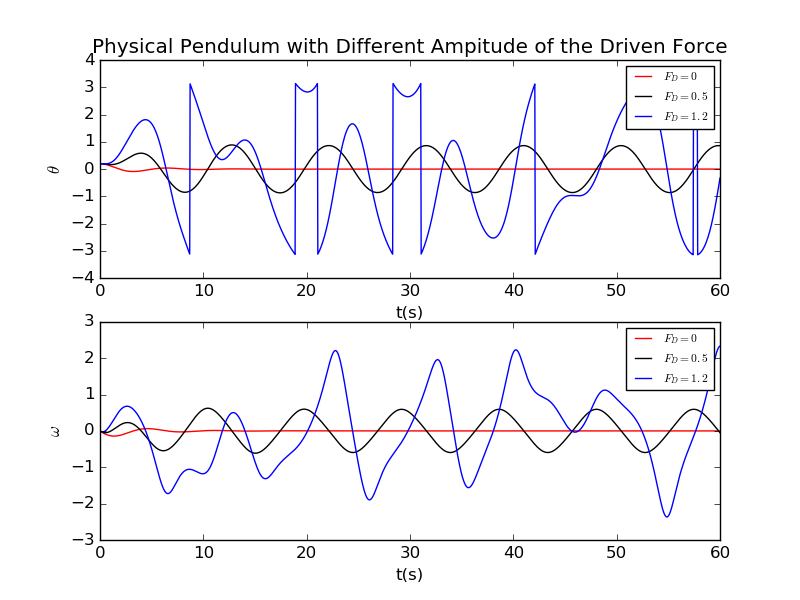
\includegraphics[width=5in]{chaotic_pend2.png}
    	\caption{Numerical Solutions}
    \end{figure}
    As we can see in the numerical plot figure, when the driven force is relatively small, the pendulum's behaviors are very much alike to normal linear pendulum. However, when the driven force is relatively large, the pendulum's motion becomes peculiar. Such motions are named \emph{chaotic motion}.\\
    The reason why this sort of motion is chaotic is that they are simultaneously deterministic and unpredictable. Given a small deviation in the initial conditions, the deviation grows exponentially with time. This property is shown in figure.2.
    \begin{figure}[htbp]
    	\centering
    	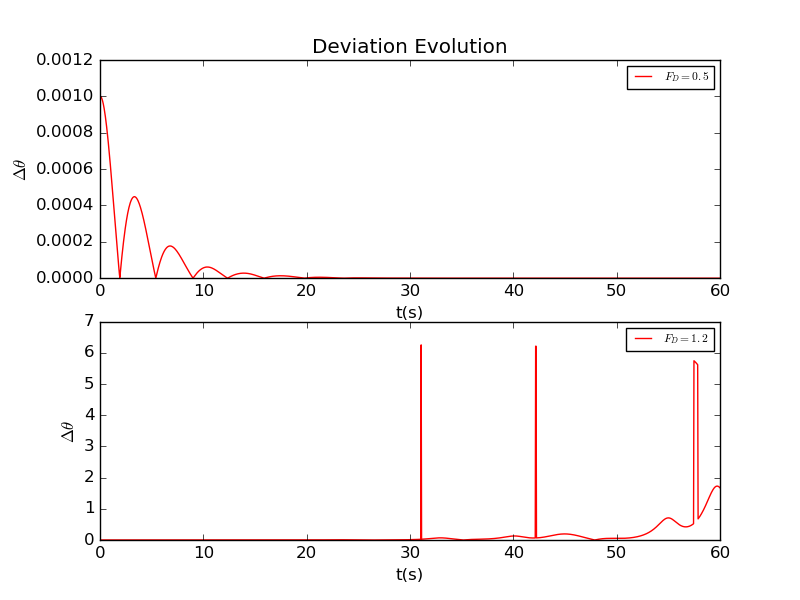
\includegraphics[width=5in]{chaotic_pend3.png}
    	\caption{Deviation Evolution}
    \end{figure}
    We notice that when $F_D=0.5$(non-chaotic motion), the deviation decays to $0$ through evolution as expected; when $F_D=1.2$(chaotic motion), the deviation grows exponentially through evolution(we should remark that the peak is mainly due to the fact that $\Delta \theta>2\pi$ and gets reset).
   \subsection{Phase Space and Poincare Section}
   Chaotic motion also has its appearance in the phase space.\\
   In our model, if the pendulum were to experience oscillation, its corresponding phase trajectory would become a simple closed curve. Chaotic motion, however, corresponds to much more exciting phase trajectory. Such comparisons are shown in figure.3.\\
    \begin{figure}[htbp]
    	\centering
    	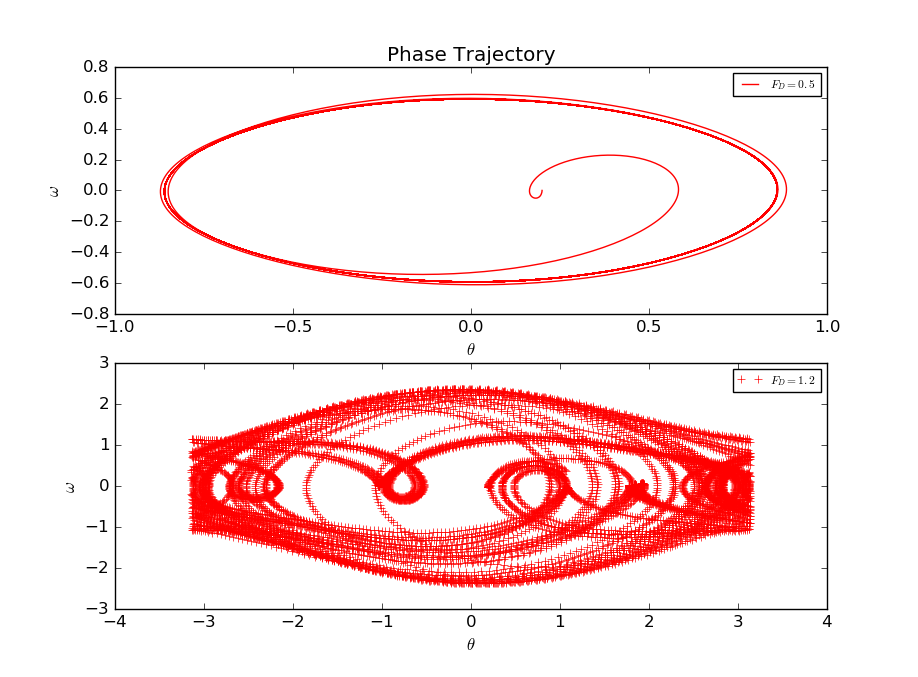
\includegraphics[width=4in]{chaotic_pend4.png}
    	\caption{Phase Trajectory}
    \end{figure}
   The chaotic motion's phase trajectory is very difficult to understand. However, we still have another method to investigate it, namely, the \emph{Poincare section}. If we only display the point when $\Omega_Dt=2n\pi$, or $\Omega_Dt=2n\pi+\pi$, or $\Omega_D=2n\pi+\pi/4$ where n is an integer. This is an example of what is know as a \emph{Poincare section}. The result is plotted in figure.4.
    \begin{figure}[htbp]
    	\centering
    	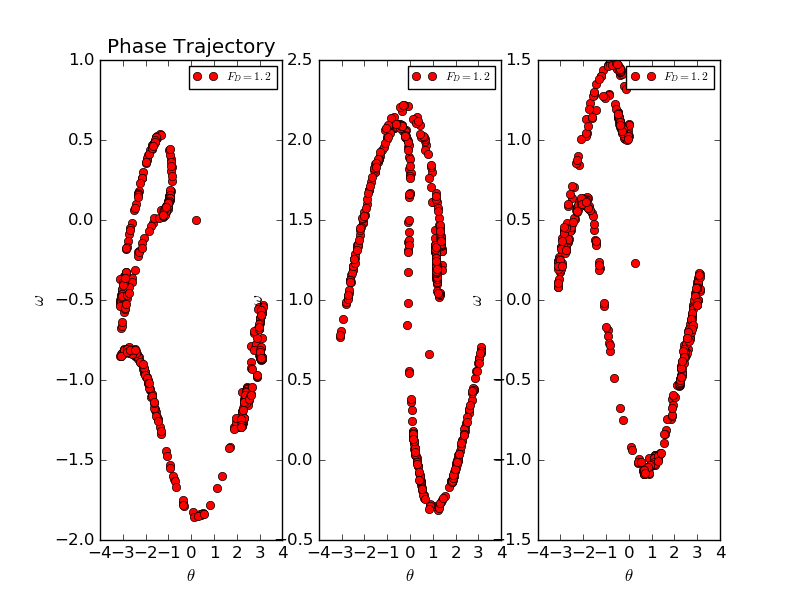
\includegraphics[width=5in]{chaotic_pend5.png}
    	\caption{Phase Trajectory;\protect\\The first figure corresponds to $\Omega_Dt=2n\pi$, the second figure corresponds to $\Omega_Dt=2n\pi+\pi$, the third figure corresponds to $\Omega_D=2n\pi+\pi/4$}
    \end{figure}
    
    \section*{Acknowledgement}
    When tackling this assignment, I benefitted a lot from the valuable discussions with Liu Xingchen. I would like to thank him for pointing out several syntax errors I made, also, for his willingness to discuss with me.
    
    \begin{thebibliography}{99}
    	\bibitem{}Hunter J, the Matplotlib Documentation, 2016
    	\bibitem{}Giordano N.J, Nakanishi H, Computational Physics, Pearson Education, 2007
    \end{thebibliography} 
\end{document}